\documentclass[conference]{IEEEtran}
% If you see 'TeX capacity exceeded' errors, try compiling with XeLaTeX or LuaLaTeX instead of pdfLaTeX.
\pdfminorversion=5
\IEEEoverridecommandlockouts

\usepackage{amssymb}
\usepackage[table]{xcolor}
\usepackage{xspace}
\usepackage{booktabs}
\usepackage{amsmath}
\usepackage{graphicx}
\usepackage{algorithm}
\usepackage{algpseudocode}
\usepackage{float}
\usepackage{placeins}
\usepackage{cite}
\usepackage{subcaption}
\usepackage{makecell}
\usepackage{xurl}
\usepackage{tikz}
\usetikzlibrary{arrows.meta, positioning, fit, calc}

% ---- Macros ----
\newcommand{\smarm}{SMARM\xspace}
\newcommand{\tdis}{$t_{\mathrm{disabled}}$\xspace}
\newcommand{\FAR}{FAR\xspace}

\begin{document}

\title{Improving Real-Time Compatibility of Shuffled Remote Attestation\\
via Atomic Copy and Memory Locking}

% DOUBLE-BLIND: comment out \author before submitting if required
\author{
  \IEEEauthorblockN{Amarin Laohajirapan, Norrathep Rattanavipanon}
  \IEEEauthorblockA{College of Computing,
    Prince of Songkla University, Phuket Campus, Thailand \\
    norrathep.r@psu.ac.th}
}

\maketitle

% ================================================================
\begin{abstract}
Remote attestation (RA) detects software compromise on IoT devices, but
classical RA keeps interrupts disabled for a full memory scan and can
block real-time work for hundreds of milliseconds.
SMARM instead measures memory in a secret shuffled order so attestation
can be interrupted between blocks while still resisting
\emph{roving malware}.
The original design was evaluated on a formally verified microkernel
stack, not on widely used production RTOSes.
We port SMARM to FreeRTOS on ARM TrustZone-M and show that, although
interrupts are re-enabled between blocks, hashing each block with
interrupts disabled still breaks common real-time periods when the block
size grows on commodity Cortex-M33 hardware.
We study two capture enhancements that keep each block snapshot atomic
while allowing HMAC work with interrupts enabled.
\emph{Atomic Copy} disables interrupts only around a short memory copy
into an isolated buffer, then hashes with interrupts enabled.
\emph{Memory locking} uses the same capture-then-hash pattern: brief
interrupt-disabled windows still required to atomically apply and tear
down the platform lock (\texttt{DSB}/\texttt{ISB} before re-enabling
interrupts), followed by in-place hashing without a copy buffer; on
TrustZone-M we implement locking via temporary SAU coverage changes.
We report \tdis for baseline hashing, Atomic Copy (memcpy), and
memory-locking lock/unlock (DWT on our prototype).
Both restore Frequency Accuracy Ratio (FAR)~$\approx 1.0$ for all tested
block sizes up to $B{=}4096$~bytes and workloads from $10$ to $1000$~Hz
on STM32L552ZE with FreeRTOS only.
\end{abstract}

\begin{IEEEkeywords}
Remote attestation, IoT security, memory locking, TrustZone-M, RTOS,
SMARM, interrupt latency
\end{IEEEkeywords}

% ================================================================
\section{Introduction}
\label{sec:intro}

IoT controllers often need both integrity checks and timely task
execution. Remote attestation
(RA)~\cite{eldefrawy2012smart,nunes2019vrased,eldefrawy2017hydra}
helps a verifier detect software compromise, but many classical designs
run the full memory measurement with interrupts off. On low-end MCUs
that window can exceed $450$~ms~\cite{nunes2019vrased}, which is
incompatible with millisecond-scale real-time loops.
\emph{Roving malware} that relocates during measurement can otherwise
evade a non-atomic scan~\cite{carpent2018smarm}.

SMARM~\cite{carpent2018smarm} addresses that threat with a different
contract: memory is measured in a one-time secret shuffled order derived
from the verifier challenge and a protected key, interrupts are allowed
\emph{between} blocks, and malware that does not know the remaining
order cannot reliably hide. The original SMARM design and analysis were
grounded in a SMART/HYDRA-style trust anchor on a formally verified
microkernel (seL4)~\cite{eldefrawy2017hydra,carpent2018smarm}. To our
knowledge it had not been ported to widely deployed production RTOSes
such as FreeRTOS. We therefore port SMARM to FreeRTOS on ARM
TrustZone-M and evaluate real-time coexistence (Section~\ref{sec:eval}).
The port shows that SMARM still fails to keep $\mathrm{FAR}\approx 1.0$
for $B\geq 2048$~bytes at a $1000$~Hz workload, because each block's
SHA-256 update remains fully non-interruptible---even though the scan as
a whole is interruptible between blocks.

This paper makes two contributions that address that remaining
bottleneck without changing SMARM's shuffled-measurement structure
against roving malware:

\begin{enumerate}
  \item \textbf{Atomic Copy.} We keep interrupts disabled only while
    copying the chosen block into a Secure-world buffer, then run
    HMAC-SHA256 with interrupts enabled. On Cortex-M33 this cuts
    \tdis by about $15\times$ versus hashing under interrupt disable,
    and restores $\mathrm{FAR}\approx 1.0$ for all evaluated block sizes.
  \item \textbf{Memory locking.} Like Atomic Copy, we keep capture
    atomic with short interrupt-disabled windows: lock the block so
    untrusted software cannot mutate it, execute \texttt{DSB}/\texttt{ISB},
    hash with interrupts enabled, then unlock under the same discipline.
    On TrustZone-M we instantiate locking by temporarily narrowing
    Non-Secure SAU coverage~\cite{armv8m-arm,an5347}. This removes the
    copy buffer and restores $\mathrm{FAR}\approx 1.0$ across all evaluated
    workloads.
\end{enumerate}

We position this paper as a self-contained study of the FreeRTOS/TrustZone-M
real-time bottleneck and the two capture mechanisms above; it is not a
shortened or extended version of other reports.
Related work discusses orthogonal companion lines on broader SMARM ports
(SMARM+)~\cite{smarmplus2026} and RTOS timekeeping during long atomic
secure execution~\cite{joianeto2026timekeeping}.

% ================================================================
\section{Background}
\label{sec:background}

\subsection{RA Atomicity and SMARM}

Classical RA often disables interrupts for the whole measurement so that
\emph{roving malware} cannot move itself while memory is being
hashed~\cite{eldefrawy2012smart,nunes2019vrased}.
SMARM~\cite{carpent2018smarm} instead derives a one-time permutation
$\sigma$ from the verifier challenge and a secret key $k$, then measures
blocks $M_{\sigma(i)}$ one by one, re-enabling interrupts between
blocks. The security claim is not ``malware cannot interrupt''; it is
that malware without knowledge of the remaining secret order cannot
reliably relocate to escape detection, and repeated independent sessions
drive the escape probability down~\cite{carpent2018smarm}.
SMARM requires three security properties:
\begin{enumerate}
  \item \textbf{(S1) Controlled Execution.}
    The attestation service is reachable only through defined
    entry/exit points (on our platform, NSC gates into Secure
    world). Interrupts may be re-enabled only
    \emph{between} block measurements---never in the middle of a
    protected capture step---so malware cannot splice itself into a
    half-measured block.
  \item \textbf{(S2) Key Secrecy.}
    The attestation key $k$ is stored in memory inaccessible to
    untrusted Non-Secure software, so malware cannot forge a valid
    report.
  \item \textbf{(S3) Private Measurement Order.}
    The permutation $\sigma$ is stored in memory inaccessible to
    KFV (known-future-visit) malware, so the adversary cannot
    predict which remaining blocks will be measured next and relocate
    ahead of the scan.
\end{enumerate}
The original SMARM evaluation used a HYDRA/seL4 trust
anchor~\cite{eldefrawy2017hydra,carpent2018smarm}. Our FreeRTOS port
keeps the same shuffled protocol and uses SMARM (interruptible between
blocks, but hash still IRQ-off per block) as the experimental baseline
against which Atomic Copy and memory locking are compared.

\subsection{TrustZone-M Isolation}
\label{sec:tz-isolation}

Cortex-M TrustZone-M~\cite{trustzone2025,armv8m-arm} splits the CPU into
Secure and Non-Secure \emph{security states}. Each memory access and
instruction fetch is checked against the Security Attribution Unit
(SAU) and the implementation-defined IDAU: enabled SAU regions mark an
address range as Non-Secure or Secure Non-Secure Callable (NSC), while
addresses not covered by any enabled region are treated as Secure by
default~\cite{an5347}. Non-Secure software cannot read or execute
Secure memory; Secure software reaches Non-Secure code only through
controlled veneers. Attestation is exported as NSC services so FreeRTOS
tasks in Non-Secure world invoke Secure measurement logic without direct
access to Secure RAM (Fig.~\ref{fig:system_model}).

Dynamic reprogramming of the SAU---as in our memory-locking
\emph{instantiation}---must be a privileged, atomic sequence: disable
interrupts; \texttt{DSB} to drain prior memory operations; update
\texttt{SAU->CTRL} and region registers as required; \texttt{DSB} and
\texttt{ISB} so subsequent instructions observe the new attribution;
then re-enable interrupts~\cite{an5347}. That sequence shortens each
IRQ-off window relative to hashing a whole block; it does \emph{not}
remove interrupt disablement around lock/unlock. The SAU governs CPU
attribution only; bus masters such as DMA may require additional
platform controls (e.g., GTZC on STM32L5)~\cite{an5347}.

We implement SMARM on the STM32L552ZE Nucleo-144 board (Cortex-M33 at
$110$~MHz). Untrusted FreeRTOS tasks run Non-Secure; the attestation
service, key $k$, and permutation $\sigma$ reside in Secure RAM and are
reachable only through NSC entries.

\begin{figure}[!t]
  \centering
  \includegraphics[width=0.92\linewidth]{system-threat-model.pdf}
  \caption{SMARM on FreeRTOS with TrustZone-M. Non-Secure tasks call the
    attestation service through NSC; key $k$ and $\sigma$ stay in Secure RAM.}
  \label{fig:system_model}
\end{figure}

Between blocks, the RTOS can preempt the Non-Secure wrapper task and run
a high-priority real-time task (Fig.~\ref{fig:workflow}).

\begin{figure}[!t]
  \centering
  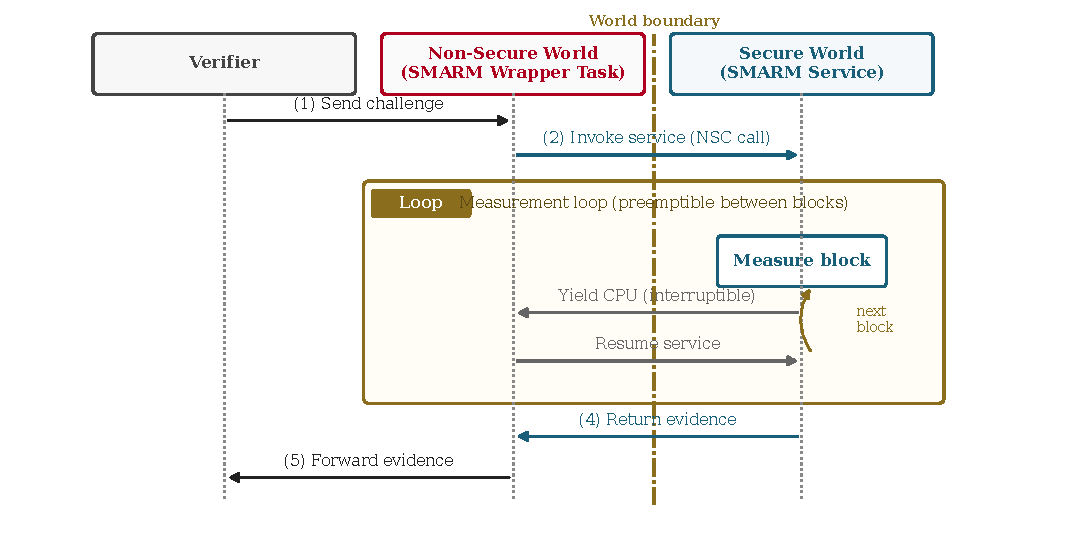
\includegraphics[width=1\linewidth]{smarm_workflow.pdf}
  \caption{End-to-end SMARM workflow. Real-time tasks may run between
    consecutive block measurements.}
  \label{fig:workflow}
\end{figure}

Table~\ref{tab:ra_comparison} places traditional RA, SMARM, and our two
enhancements side by side.

\begin{table}[!t]
  \centering
  \caption{Comparison of attestation approaches for real-time IoT devices.}
  \label{tab:ra_comparison}
  \renewcommand{\arraystretch}{1.1}
  \small
  \setlength{\tabcolsep}{2.5pt}
  \begin{tabular}{lcccc}
    \toprule
    \textbf{Approach} &
    \textbf{RT-safe} &
    \makecell{\textbf{Extra} \\ \textbf{RAM}} &
    \makecell{\textbf{Atomic} \\ \textbf{window}} &
    \textbf{RTOS} \\
    \midrule
    Traditional RA~\cite{eldefrawy2012smart} &
      \texttimes & 0 & Full scan & \texttimes \\
    SMARM~\cite{carpent2018smarm} &
      Partial & 0 & Per-block hash & \texttimes \\
    \textbf{Atomic Copy} &
      \checkmark & $+B$ & Per-block copy & \checkmark \\
    \textbf{Memory locking} &
      \checkmark & 0 & Lock+barriers & \checkmark \\
    \bottomrule
  \end{tabular}
\end{table}

% ================================================================
\section{Motivation}
\label{sec:motivation}

In baseline SMARM, each block update disables interrupts for the full
SHA-256 work on that block. With about $1.1$~MB/s hash throughput on our
board, \tdis grows from $0.062$~ms at $B{=}64$~bytes to $3.75$~ms at
$B{=}4096$~bytes. For a $1000$~Hz real-time task, the activation period
is only $1$~ms, so a single large-block hash can span several periods
and force the scheduler to miss multiple deadlines in a row. The problem
is therefore not that SMARM allows interrupts between blocks---that
property is intentional---but that the \emph{within-block} hash still
runs as one long non-preemptible critical section whose duration scales
linearly with~$B$.

Figure~\ref{fig:timing_diagram} sketches the interrupt-disabled windows
for traditional RA, SMARM baseline, and Atomic Copy. Traditional RA
keeps interrupts off for the entire scan; SMARM shortens that window to
one block hash; Atomic Copy shortens it further to one block copy.

\begin{figure}[!t]
  \centering
  \includegraphics[width=\linewidth]{timing_diagram.png}
  \caption{Interrupt-disabled windows. Traditional RA covers the full
    scan. SMARM limits disability to one block hash. Atomic Copy further
    limits it to one block copy.}
  \label{fig:timing_diagram}
\end{figure}

Figure~\ref{fig:setup_and_baseline_far} shows the measured impact on
real-time availability. Under a $1000$~Hz workload, $\mathrm{FAR}$ stays
near $1.0$ only for $B\leq 1024$~bytes and falls sharply at
$B\geq 2048$~bytes (down to about $0.27$ at $B{=}4096$). In other
words, baseline SMARM coexists well with millisecond-scale control loops
only when blocks are small; once block hashing exceeds the task period,
attestation directly degrades the timing behavior that many IoT
controllers depend on.

\begin{figure}[!t]
  \centering
  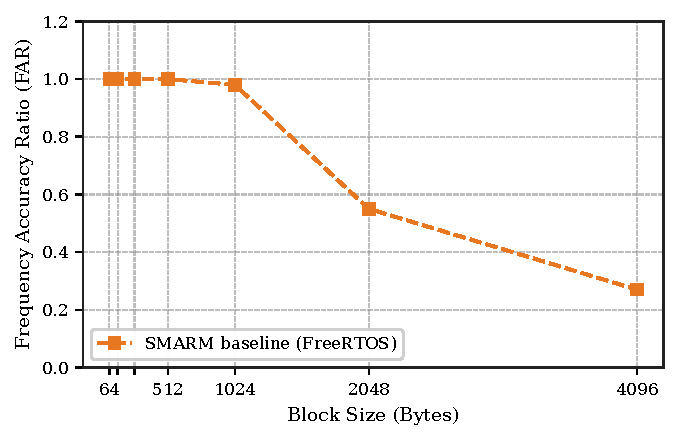
\includegraphics[width=\linewidth]{far_1000.pdf}
  \caption{FAR of baseline SMARM under a $1000$~Hz real-time workload
    across block sizes (FreeRTOS). Values stay near $1.0$ for
    $B\leq 1024$~bytes and drop for larger $B$.}
  \label{fig:setup_and_baseline_far}
\end{figure}

\textbf{Root cause and design opportunity.}
The baseline fails real-time coexistence not because shuffled
attestation is inherently non-interruptible, but because each block hash
currently runs with interrupts disabled for too long relative to common
RTOS periods. This is an engineering bottleneck introduced by how the
baseline port protects block integrity, not a requirement of SMARM's
security argument against roving malware. Cryptographic hashing itself
can proceed with interrupts enabled once the bytes fed to HMAC form a
consistent snapshot. What must remain atomic is only the \emph{capture}
of those bytes: malware must not be able to splice a block while it is
being read for measurement. Section~\ref{sec:design} builds on that
distinction and presents two capture mechanisms---Atomic Copy and
memory locking---that keep capture atomic while restoring interruptible
hash work and FAR~$\approx 1.0$ across the block sizes we evaluate.

\FloatBarrier
% ================================================================
\section{Design}
\label{sec:design}

\subsection{Atomic Copy}
\label{sec:atomic}

Atomic Copy splits each block step into (i)~an interrupt-disabled
\texttt{Memcpy} into a Secure buffer of size $B$, and (ii)~an
interrupt-enabled \texttt{HMAC.Update} over that buffer
(Fig.~\ref{fig:atomic_copy_workflow}, Algorithm~\ref{alg:atomic_copy}).
Memory copy on our Cortex-M33 is about $17$~MB/s, so
$t_{\mathrm{disabled}}^{\mathrm{copy}}\approx B/17\,\mathrm{MB/s}$,
roughly $15\times$ shorter than hashing under interrupt disable.

\begin{figure}[!t]
  \centering
  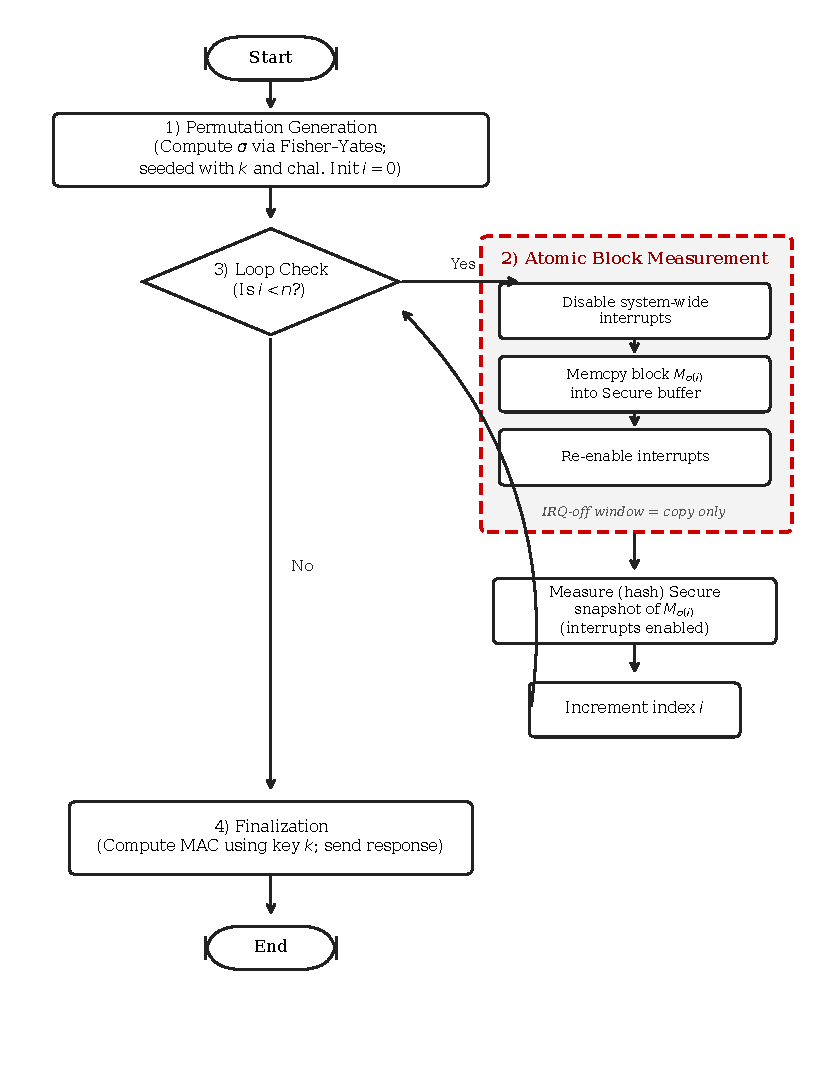
\includegraphics[width=\linewidth,height=0.24\textheight,keepaspectratio]{atomic_workflow.pdf}
  \caption{Atomic Copy flowchart. The dashed region is the short
    interrupt-disabled window (copy only); hashing runs afterward with
    interrupts enabled.}
  \label{fig:atomic_copy_workflow}
\end{figure}

\begin{algorithm}[t]
\caption{Atomic Copy Secure Service}
\label{alg:atomic_copy}
\begin{algorithmic}[1]
\Require $n$ blocks, shuffled indices $\sigma$, memory $M$, key $k$
\State \Call{HMAC.Init}{$k$}
\For{$i \gets 0$ to $n-1$}
  \State $\mathit{blk} \gets M[\sigma(i)\cdot B]$
  \State \Call{DisableInterrupts}{}
  \State \Call{Memcpy}{\textit{buf}, \textit{blk}, $B$} \Comment{atomic snapshot}
  \State \Call{EnableInterrupts}{}
  \State \Call{HMAC.Update}{\textit{buf}, $B$} \Comment{interrupts on}
\EndFor
\State \textbf{return} \Call{HMAC.Finalize}{}
\end{algorithmic}
\end{algorithm}

\textbf{Security sketch.} The IRQ-off window covers only the copy, so
the snapshot that feeds HMAC is not half-updated~(S1). Key $k$ and
permutation $\sigma$ remain in Secure RAM~(S2)--(S3); hashing after the
copy uses only Secure buffer contents. We summarize preservation of
(S1)--(S3) for both designs in Section~\ref{sec:security_summary}.

\subsection{Memory Locking}
\label{sec:memory-locking}

Atomic Copy requires an extra buffer of size $B$. \emph{Memory locking}
avoids copying by atomically changing how the platform exposes the
selected block to untrusted software: once locked, the adversary cannot
lawfully read or write that block during HMAC, so hashing can proceed
with interrupts enabled---the same capture-then-hash structure as Atomic
Copy, but capture is a \emph{lock} rather than \texttt{Memcpy}.

Locking does \emph{not} eliminate interrupt disablement. Each lock and
unlock must be atomic: disable interrupts, apply the platform lock,
drain prior accesses with \texttt{DSB}, reprogram protection state if
needed, re-enable the protection unit, then \texttt{DSB} and \texttt{ISB}
before enabling interrupts again (Fig.~\ref{fig:sau_workflow},
Algorithm~\ref{alg:memlock}). Per block we perform one locked window for
hashing and restore the prior mapping afterward.

\begin{algorithm}[t]
\caption{Memory Locking Secure Service (platform-neutral)}
\label{alg:memlock}
\begin{algorithmic}[1]
\Require $n$ blocks, shuffled indices $\sigma$, memory $M$, key $k$
\State \Call{HMAC.Init}{$k$}
\State \Call{UnlockAll}{$M$} \Comment{rest state}
\For{$i \gets 0$ to $n-1$}
  \State $\mathit{blk} \gets M[\sigma(i)\cdot B]$
  \State \Call{DisableInterrupts}{}
  \State \Call{DSB}{}
  \State \Call{LockBlock}{\textit{blk}, $B$}
  \State \Call{DSB}{}; \Call{ISB}{}
  \State \Call{EnableInterrupts}{}
  \State \Call{HMAC.Update}{\textit{blk}, $B$} \Comment{interrupts on}
  \State \Call{DisableInterrupts}{}
  \State \Call{DSB}{}
  \State \Call{UnlockAll}{$M$}
  \State \Call{DSB}{}; \Call{ISB}{}
  \State \Call{EnableInterrupts}{}
\EndFor
\State \textbf{return} \Call{HMAC.Finalize}{}
\end{algorithmic}
\end{algorithm}

\begin{figure}[!t]
  \centering
  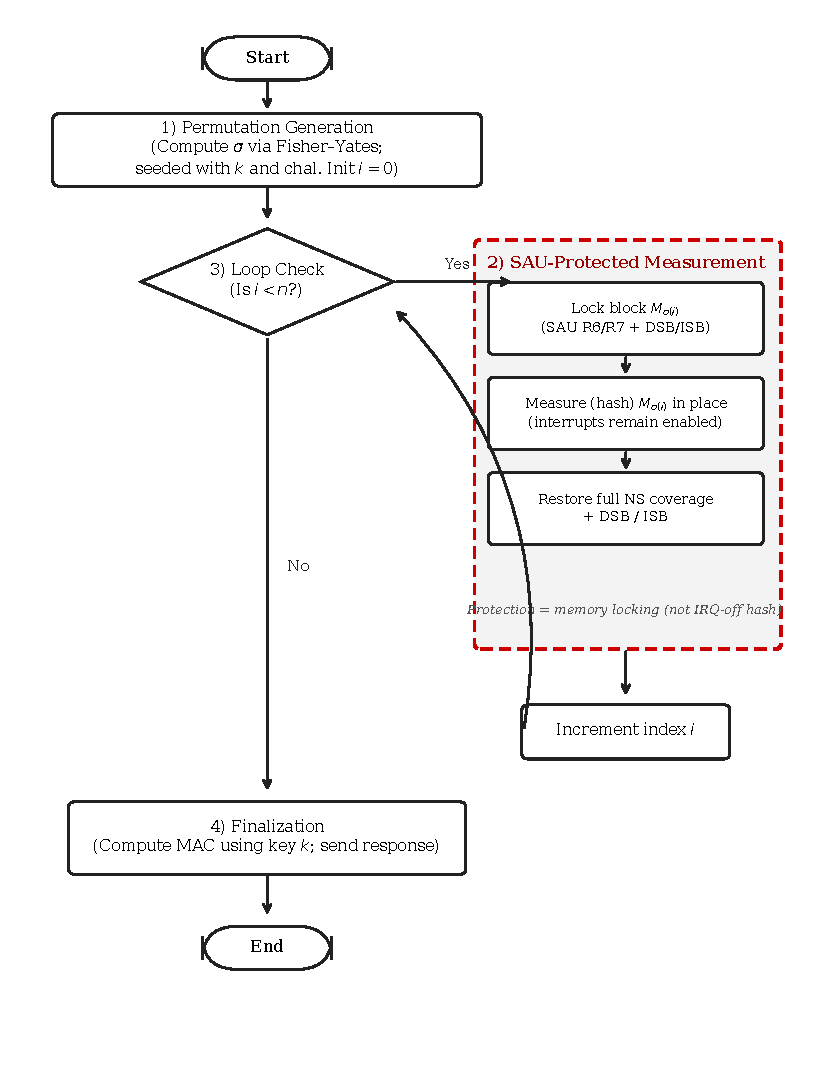
\includegraphics[width=\linewidth,height=0.24\textheight,keepaspectratio]{sau_workflow.pdf}
  \caption{Memory locking flowchart (TrustZone-M prototype). Dashed
    regions: interrupt-disabled lock/unlock with \texttt{DSB}/\texttt{ISB};
    hashing runs with interrupts enabled.}
  \label{fig:sau_workflow}
\end{figure}

\subsubsection{TrustZone-M instantiation}
\label{sec:sau}

On Cortex-M TrustZone-M, \Call{LockBlock}{} can reprogram the Security
Attribution Unit (SAU): enabled regions mark ranges as Non-Secure or
Secure+NSC, and addresses not covered by any enabled region are Secure
\emph{by default}~\cite{armv8m-arm,an5347}. We temporarily narrow
Non-Secure coverage in a dedicated attested data window so only the
fragments before and after the selected block remain Non-Secure; the
block is uncovered and therefore locked for in-place HMAC
(Fig.~\ref{fig:sau_memory_map}). Regions~6/7 implement split coverage;
region~1 keeps Non-Secure application code separate.

\begin{figure}[!t]
  \centering
  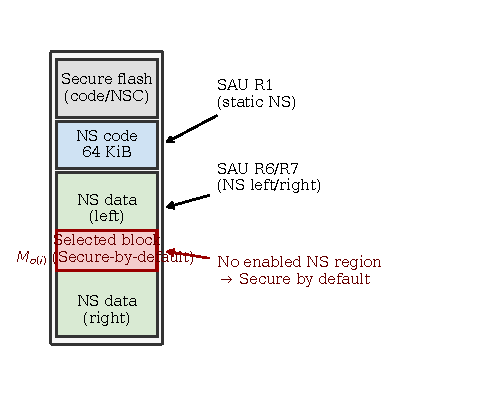
\includegraphics[width=\linewidth]{sau_memory_map.pdf}
  \caption{TrustZone-M memory locking (SAU-based). The selected block is
    Secure by default while surrounding bytes stay Non-Secure.}
  \label{fig:sau_memory_map}
\end{figure}

Our prototype follows the barrier discipline recommended for dynamic SAU
updates: disable interrupts, \texttt{DSB}, optionally toggle
\texttt{SAU->CTRL}, configure region registers, re-enable the SAU,
\texttt{DSB}, \texttt{ISB}, then enable interrupts. CPU attribution via
SAU suffices when no bus master concurrently accesses the attested
window; DMA/GTZC and post-boot SAU locking on TF-M-style images are
discussed in Section~\ref{sec:guidance}. The attested window lies in
Non-Secure flash outside application code/vectors.

\textbf{Security sketch.} Locking makes the block inaccessible to
Non-Secure software during hashing~(S1); lock/unlock remain atomic via
interrupt disable and barriers. Key $k$ and $\sigma$ stay in Secure
RAM~(S2)--(S3). Section~\ref{sec:security_summary} summarizes both
designs.

\subsection{Security Properties Preserved}
\label{sec:security_summary}

Atomic Copy and memory locking change \emph{how} each block is captured
for hashing; they do not change SMARM's cryptographic protocol or the
placement of secrets. Both designs therefore preserve
(S1)--(S3):
\begin{itemize}
  \item \textbf{(S1) Controlled Execution.}
    Attestation still runs only through Secure/NSC entry points.
    Between blocks, interrupts remain enabled as in SMARM.
    Within a block, Atomic Copy keeps interrupts disabled for the
    entire \texttt{Memcpy}, and memory locking keeps interrupts disabled
    only for each lock/unlock sequence (with \texttt{DSB}/\texttt{ISB}),
    then denies Non-Secure access to the locked block while hashing with
    interrupts enabled. In either case, untrusted software cannot splice
    into a half-captured measurement.
  \item \textbf{(S2) Key Secrecy.}
    The HMAC key $k$ never leaves Secure RAM; neither design exposes
    $k$ to Non-Secure code or to the attested data window.
  \item \textbf{(S3) Private Measurement Order.}
    The permutation $\sigma$ is derived and stored in Secure world and
    is never written to Non-Secure memory. Malware therefore still
    cannot learn the remaining visit order.
\end{itemize}
In short, Atomic Copy and memory locking reduce the real-time cost of
block capture while retaining SMARM's controlled execution and the
secrecy of $k$ and $\sigma$.

\FloatBarrier
% ================================================================
\section{Evaluation}
\label{sec:eval}

\subsection{Setup}
\label{sec:eval-setup}

All results use STM32L552ZE at $110$~MHz with FreeRTOS only.
Block sizes are $B\in\{64,128,256,512,1024,2048,4096\}$~bytes.
For baseline SMARM and Atomic Copy, attested memory is $512$~KB of
Non-Secure flash as in our port of the original protocol.
For \emph{memory locking} we use a dedicated $128$~KB Non-Secure data
window at $0\mathrm{x}08060000$--$0\mathrm{x}0807FFFF$, preceded by a
$64$~KB guard gap ($0\mathrm{x}08050000$--$0\mathrm{x}0805FFFF$) that
is not measured, and a separate $64$~KB Non-Secure application region
so dynamic SAU updates never overlap application vectors or text.

\textbf{FAR metric.}
We report real-time availability as
$\mathrm{FAR}=f_{\mathrm{observed}}/f_{\mathrm{baseline}}$, where
$f_{\mathrm{observed}}$ is the frequency of a high-priority real-time
task during attestation and $f_{\mathrm{baseline}}$ is its frequency
without attestation. Values near $1.0$ mean little interference; values
below $1.0$ indicate missed activations. We drive the real-time task at
$1000$, $100$, and $10$~Hz during memory-locking sweeps ($21$
configurations). At $1000$~Hz, UART summaries report
$\mathrm{FAR}\in[1.000,1.008]$ on some warm-up rounds because of tick
alignment while attestation still meets every deadline; we therefore
summarize memory locking as $\mathrm{FAR}\approx 1.0$ with no observed
$\mathrm{FAR}<1$. At $100$ and $10$~Hz the attestation window often
spans multiple task periods, so integer counting can yield
$\mathrm{FAR}>1$ even without starvation; we treat that as a metric
artifact, not improved real-time performance.

We report: (i)~TIM2-based \tdis for baseline SMARM and Atomic Copy,
(ii)~DWT cycle counts for memory-locking lock+unlock per block (TrustZone-M
SAU prototype, interrupts disabled around each transition with
\texttt{DSB}/\texttt{ISB}), and (iii)~\FAR as above. We omit end-to-end
runtime comparisons between $512$~KB baseline/Atomic runs and the
$128$~KB locking window because they would conflate algorithmic cost
with attested size.

\subsection{Non-Interruptibility Cost}

Table~\ref{tab:tdisabled} recalls Atomic Copy versus baseline SMARM.
Atomic Copy reduces \tdis by about $15$--$16\times$ for
$B\geq 128$~bytes because only the copy---not the hash---runs with
interrupts disabled.

\begin{table}[!t]
  \centering
  \small
  \caption{$t_{\mathrm{disabled}}$: SMARM baseline vs.\ Atomic Copy
    (TIM2, FreeRTOS). Std.\ $<0.003$~ms.}
  \label{tab:tdisabled}
  \setlength{\tabcolsep}{3.5pt}
  \begin{tabular}{rrrrr}
    \toprule
    & \multicolumn{2}{c}{\textbf{Baseline}}
    & \multicolumn{2}{c}{\textbf{Atomic Copy}} \\
    \cmidrule(lr){2-3}\cmidrule(lr){4-5}
    \textbf{$B$} & Mean (ms) & Std & Mean (ms) & Std \\
    \midrule
    64   & 0.062 & 0.001 & $<$0.007$^\dagger$ & --- \\
    128  & 0.120 & 0.001 & 0.007 & --- \\
    256  & 0.237 & 0.001 & 0.015 & --- \\
    512  & 0.472 & 0.002 & 0.029 & --- \\
    1024 & 0.939 & 0.001 & 0.058 & --- \\
    2048 & 1.877 & 0.003 & 0.116 & --- \\
    4096 & 3.749 & 0.002 & 0.240 & --- \\
    \bottomrule
  \end{tabular}

  \smallskip
  \raggedright\footnotesize
  $^\dagger$Completes within one TIM2 tick ($7.27\,\mu$s).
\end{table}

\textbf{Memory locking.} Per block, \tdis comprises two
interrupt-disabled intervals (lock and unlock), each including platform
lock programming plus \texttt{DSB}/\texttt{ISB}. The HMAC update runs
with interrupts enabled, so hashing time does not add to the IRQ-off
budget. Table~\ref{tab:tdis_lock} summarizes DWT cycle counts for
lock+unlock on our TrustZone-M SAU implementation (both sequences
combined, firmware with interrupt disable and barriers enforced). Cycles
grow modestly with~$B$ ($87$--$143$) because the SAU hole spans more
address space, but remain $\ll 0.01$~ms at $110$~MHz---orders of
magnitude below baseline per-block hashing in Table~\ref{tab:tdisabled}.

\begin{table}[!t]
  \centering
  \small
  \caption{Memory locking \tdis: DWT cycles per block (lock+unlock,
    TrustZone-M SAU prototype, mean $\pm$ std over $10$ rounds).}
  \label{tab:tdis_lock}
  \setlength{\tabcolsep}{4pt}
  \begin{tabular}{rrr}
    \toprule
    \textbf{$B$ (bytes)} & \textbf{Mean cycles} & \textbf{Std} \\
    \midrule
    64   & 87.0 & 0.0 \\
    128  & 88.0 & 0.0 \\
    256  & 90.0 & 0.0 \\
    512  & 93.9 & 0.3 \\
    1024 & 100.9 & 0.3 \\
    2048 & 114.7 & 0.5 \\
    4096 & 142.9 & 0.7 \\
    \bottomrule
  \end{tabular}
\end{table}

\subsection{Real-Time Availability}

Figure~\ref{fig:far_three} summarizes FAR at $1000$~Hz. Baseline SMARM
degrades for large $B$, whereas Atomic Copy and memory locking remain at
$\mathrm{FAR}\approx 1.0$ through $B{=}4096$~bytes. Memory locking was
swept across all seven block sizes at $10$, $100$, and $1000$~Hz
($21$ configurations) with interrupt disable and \texttt{DSB}/\texttt{ISB}
around each lock/unlock; we observed no $\mathrm{FAR}<1$ (no missed
deadlines). At $1000$~Hz, $\mathrm{FAR}=1.000$ in steady-state rounds;
at lower rates, integer counting occasionally reports
$\mathrm{FAR}>1$ when attestation spans multiple periods
(Section~\ref{sec:eval-setup}).

\begin{figure}[!htbp]
  \centering
  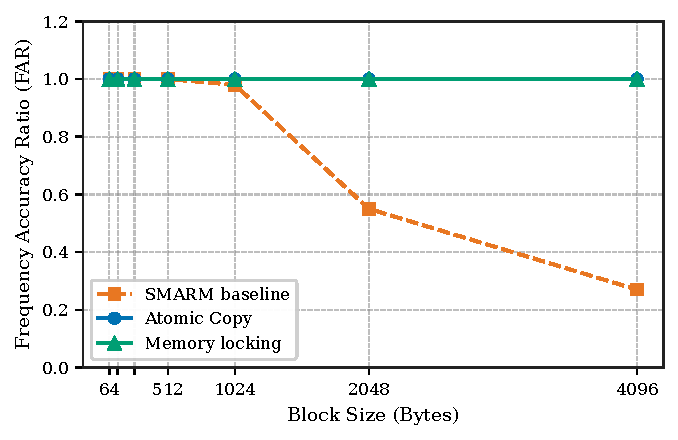
\includegraphics[width=\linewidth]{far_three_1000hz.pdf}
  \caption{FAR under a $1000$~Hz workload. Baseline SMARM loses
    activations for large blocks, whereas Atomic Copy and memory locking
    maintain FAR~$\approx 1.0$.}
  \label{fig:far_three}
\end{figure}

\subsection{Storage Overhead}

Atomic Copy needs one Secure buffer of size $B$ (up to $4$~KB at
$B{=}4096$). Memory locking needs no extra measurement buffer. Both keep
$k$ and $\sigma$ in Secure RAM as in baseline SMARM.
Table~\ref{tab:storage} summarizes the trade-off: Atomic Copy pays a
small, predictable Secure RAM cost; memory locking avoids that buffer but
requires a dedicated Non-Secure data window disjoint from application
code (SAU instantiation).

\begin{table}[H]
  \centering
  \small
  \caption{Storage and layout overhead of the two enhancements.}
  \label{tab:storage}
  \setlength{\tabcolsep}{3.5pt}
  \begin{tabular}{lcc}
    \toprule
    \textbf{Item} & \textbf{Atomic Copy} & \textbf{Mem.\ locking} \\
    \midrule
    Secure copy buffer & $+B$ (up to $4$~KB) & none \\
    Extra Secure secrets & $k$, $\sigma$ & $k$, $\sigma$ \\
    Dedicated attested window & not required & $128$~KB (NS flash) \\
    Dynamic SAU regions & none & regions~6/7 \\
    \bottomrule
  \end{tabular}
\end{table}

\subsection{Summary and Design Guidance}
\label{sec:guidance}

Table~\ref{tab:metric_summary} compresses the evaluation into three axes.
Baseline SMARM fails FAR for large $B$ because hashing remains
interrupt-disabled. Both enhancements restore FAR~$\approx 1.0$, but they
pay different costs: Atomic Copy shortens the IRQ-off window to a copy
and consumes Secure RAM of size $B$; memory locking uses two brief
IRQ-off windows per block for lock/unlock (TrustZone-M: SAU +
\texttt{DSB}/\texttt{ISB}), keeps hashing interruptible, and requires a
dedicated Non-Secure data window.

\begin{table}[H]
  \centering
  \footnotesize
  \caption{Summary of the three SMARM variants on FreeRTOS/TrustZone-M.}
  \label{tab:metric_summary}
  \setlength{\tabcolsep}{2.5pt}
  \renewcommand{\arraystretch}{1.12}
  \begin{tabular*}{\columnwidth}{@{\extracolsep{\fill}}lccc@{}}
    \toprule
    & \textbf{FAR} &
    \makecell{\textbf{IRQ-off}\\\textbf{window}} &
    \makecell{\textbf{RAM /}\\\textbf{layout}} \\
    \midrule
    SMARM baseline &
      Drops at large $B$ &
      Per-block hash &
      No extra buffer \\
    Atomic Copy &
      $\approx 1.0$ &
      Per-block copy &
      $+B$ buffer \\
    Memory locking &
      $\approx 1.0$ &
      2$\times$ lock+barriers &
      NS data window \\
    \bottomrule
  \end{tabular*}
\end{table}

\textbf{When to prefer each enhancement.}
Platform guidance typically configures SAU once at boot as part of the
static Secure/Non-Secure map~\cite{armv8m-arm,an5347,cmsis-tz,tfm-isolation},
and production TF-M-style images often lock SAU/GTZC after that
setup~\cite{um2851,tfm2024}. Our TrustZone-M \emph{instantiation} using the SAU is not a replacement
for that static partition: it is a short, Secure-only change to a
dedicated data window during attestation.
Choose as follows:

\begin{itemize}
  \item \textbf{Atomic Copy} when Secure RAM of size $B$ is available,
    when SAU must remain locked after boot, when free SAU regions are
    scarce, or when the attested image cannot be isolated from Non-Secure
    code/vectors.
  \item \textbf{Memory locking} (SAU on TrustZone-M) when Secure RAM is
    tight, a dedicated Non-Secure data window can be reserved, and Secure
    software is allowed to reprogram SAU briefly. Because SAU/IDAU govern
    attribution only, DMA or other bus masters still need platform
    controls such as GTZC~\cite{an5347}.
\end{itemize}
The conference prototype leaves SAU unlocked so Non-Secure coverage can
be narrowed and restored during attestation; locking policy and DMA-aware enforcement are left to the
extended version.

% ================================================================
\section{Related Work}
\label{sec:related}

\textbf{Classical and shuffled RA.}
SMART~\cite{eldefrawy2012smart}, VRASED~\cite{nunes2019vrased}, and
HYDRA~\cite{eldefrawy2017hydra} use long atomic measurements.
SMARM~\cite{carpent2018smarm}, PRoM~\cite{aman2021prom}, and
HAtt~\cite{aman2018hatt} use shuffled measurement to resist roving
malware while allowing interrupts between blocks. SMARM's original
prototype targeted a seL4/HYDRA stack rather than commodity RTOSes; our
baseline is a FreeRTOS/TrustZone-M port of that protocol, against which
we evaluate Atomic Copy and memory locking (this paper's scope).
Broader ports and storage-oriented variants appear in SMARM+~\cite{smarmplus2026}.

\textbf{Interruptible attestation.}
ISC-FLAT~\cite{isc-flat}, ASAP~\cite{asap}, and IDA~\cite{ida2024}
handle interrupts in control-flow or hybrid attestation. They are
complementary; we target memory-content RA under FreeRTOS.

\textbf{RTOS timekeeping vs.\ atomic secure execution.}
Joia Neto et al.~\cite{joianeto2026timekeeping} characterize a
distinct facet of the same underlying conflict on TrustZone-M: while
Non-Secure interrupts are masked for an atomic secure service, the
NVIC delivers at most one pending SysTick, so the Non-Secure RTOS
under-counts ticks and drifts from wall-clock time (prior work reports
this on FreeRTOS and Zephyr~\cite{joianeto2026timekeeping}); remote
attestation is among the evaluated atomic services.
They reconcile this by handling SysTick from the Secure World and
reconstructing timer-visible kernel state without modifying the RTOS.
Our work is orthogonal: Atomic Copy and memory locking \emph{shorten}
each SMARM block's interrupt-disabled capture window so periodic
real-time activations remain accurate under a FAR-style metric, rather
than compensating the kernel after a long atomic hash.
The two directions can be combined on the same platform.

\textbf{TrustZone-M and SAU.}
TrustZone-M and SAU define CPU security
attribution~\cite{trustzone2025,armv8m-arm,an5347,cmsis-tz}. TF-M and
vendor TFM examples usually set a static SAU map early and may lock it
until reset~\cite{tfm2024,tfm-isolation,um2851}. We instantiate memory
locking on TrustZone-M via brief dynamic SAU updates as an alternative
to copying a block into Secure RAM during SMARM measurement, and discuss
when that choice is appropriate in Section~\ref{sec:guidance}.

\textbf{Custom hardware.}
LO-FAT~\cite{lo-fat}, LiteHAX~\cite{litehax}, and ATRIUM~\cite{atrium}
remove non-interruptible windows with dedicated hardware. We stay on
unmodified TrustZone-M MCUs.

% ================================================================
\section{Conclusion}
\label{sec:conclusion}

SMARM improves RA interactivity, but interrupt-disabled hashing still
hurts FAR for large blocks on FreeRTOS/TrustZone-M. Atomic Copy cuts
that window to a memory copy and restores FAR~$\approx 1.0$ with a
buffer of size $B$. Memory locking uses the same capture-then-hash
structure with brief IRQ-off lock/unlock (TrustZone-M: SAU +
\texttt{DSB}/\texttt{ISB}) instead of \texttt{Memcpy}, avoids a copy
buffer, and keeps FAR~$\approx 1.0$ across all tested block sizes and
$10$--$1000$~Hz workloads. Both enhancements preserve SMARM's
security properties~(S1)--(S3): controlled Secure/NSC entry with
integrity of each block capture, secrecy of $k$, and privacy of the
measurement order~$\sigma$. In practice, prefer Atomic Copy when
Secure RAM is available or SAU must stay locked, and prefer memory
locking when a dedicated Non-Secure data window can absorb temporary
attribution changes without an extra Secure buffer.

\bibliographystyle{IEEEtran}
\bibliography{citation}

\end{document}
